% Created by tikzDevice version 0.8.1 on 2015-11-17 12:15:23
% !TEX encoding = UTF-8 Unicode
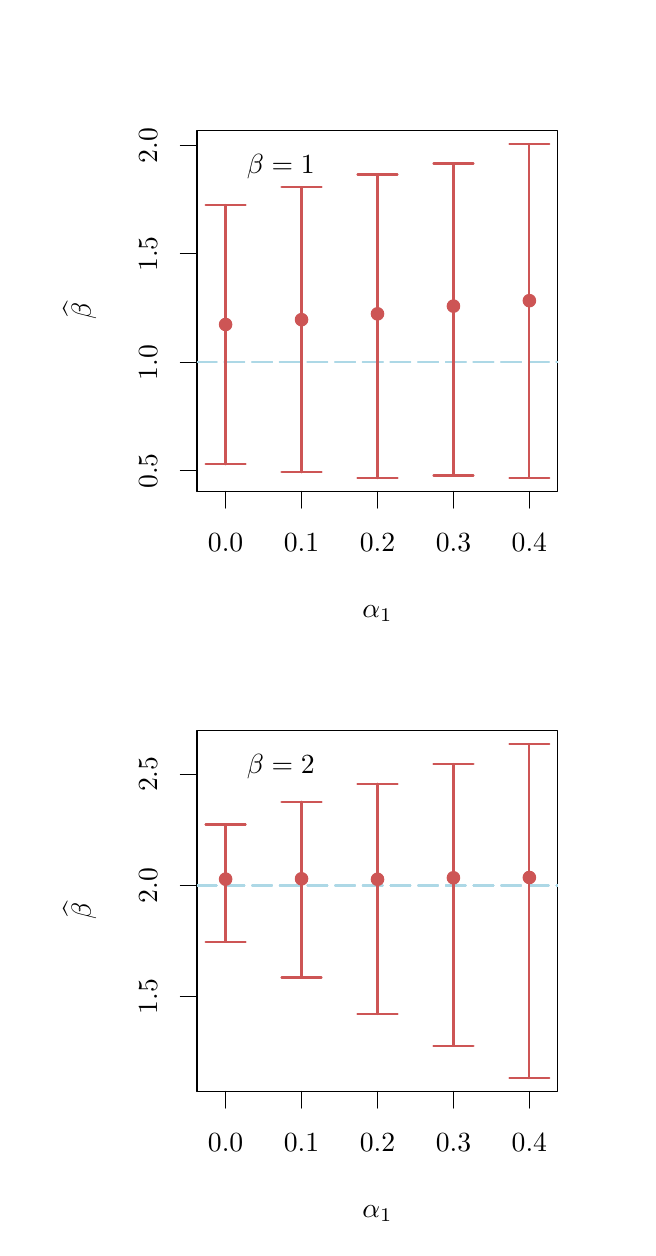
\begin{tikzpicture}[x=1pt,y=1pt]
\definecolor{fillColor}{RGB}{255,255,255}
\path[use as bounding box,fill=fillColor,fill opacity=0.00] (0,0) rectangle (216.81,433.62);
\begin{scope}
\path[clip] ( 61.20,266.01) rectangle (191.61,396.42);
\definecolor{drawColor}{RGB}{255,255,255}
\definecolor{fillColor}{RGB}{255,255,255}

\path[draw=drawColor,line width= 0.4pt,line join=round,line cap=round,fill=fillColor] ( 71.52,326.36) circle (  2.25);

\path[draw=drawColor,line width= 0.4pt,line join=round,line cap=round,fill=fillColor] ( 98.96,328.10) circle (  2.25);

\path[draw=drawColor,line width= 0.4pt,line join=round,line cap=round,fill=fillColor] (126.41,330.21) circle (  2.25);

\path[draw=drawColor,line width= 0.4pt,line join=round,line cap=round,fill=fillColor] (153.85,333.00) circle (  2.25);

\path[draw=drawColor,line width= 0.4pt,line join=round,line cap=round,fill=fillColor] (181.29,334.97) circle (  2.25);
\end{scope}
\begin{scope}
\path[clip] (  0.00,  0.00) rectangle (216.81,433.62);
\definecolor{drawColor}{RGB}{0,0,0}

\path[draw=drawColor,line width= 0.4pt,line join=round,line cap=round] ( 71.52,266.01) -- (181.29,266.01);

\path[draw=drawColor,line width= 0.4pt,line join=round,line cap=round] ( 71.52,266.01) -- ( 71.52,260.01);

\path[draw=drawColor,line width= 0.4pt,line join=round,line cap=round] ( 98.96,266.01) -- ( 98.96,260.01);

\path[draw=drawColor,line width= 0.4pt,line join=round,line cap=round] (126.41,266.01) -- (126.41,260.01);

\path[draw=drawColor,line width= 0.4pt,line join=round,line cap=round] (153.85,266.01) -- (153.85,260.01);

\path[draw=drawColor,line width= 0.4pt,line join=round,line cap=round] (181.29,266.01) -- (181.29,260.01);

\node[text=drawColor,anchor=base,inner sep=0pt, outer sep=0pt, scale=  1.00] at ( 71.52,244.41) {0.0};

\node[text=drawColor,anchor=base,inner sep=0pt, outer sep=0pt, scale=  1.00] at ( 98.96,244.41) {0.1};

\node[text=drawColor,anchor=base,inner sep=0pt, outer sep=0pt, scale=  1.00] at (126.41,244.41) {0.2};

\node[text=drawColor,anchor=base,inner sep=0pt, outer sep=0pt, scale=  1.00] at (153.85,244.41) {0.3};

\node[text=drawColor,anchor=base,inner sep=0pt, outer sep=0pt, scale=  1.00] at (181.29,244.41) {0.4};

\path[draw=drawColor,line width= 0.4pt,line join=round,line cap=round] ( 61.20,273.47) -- ( 61.20,391.09);

\path[draw=drawColor,line width= 0.4pt,line join=round,line cap=round] ( 61.20,273.47) -- ( 55.20,273.47);

\path[draw=drawColor,line width= 0.4pt,line join=round,line cap=round] ( 61.20,312.68) -- ( 55.20,312.68);

\path[draw=drawColor,line width= 0.4pt,line join=round,line cap=round] ( 61.20,351.88) -- ( 55.20,351.88);

\path[draw=drawColor,line width= 0.4pt,line join=round,line cap=round] ( 61.20,391.09) -- ( 55.20,391.09);

\node[text=drawColor,rotate= 90.00,anchor=base,inner sep=0pt, outer sep=0pt, scale=  1.00] at ( 46.80,273.47) {0.5};

\node[text=drawColor,rotate= 90.00,anchor=base,inner sep=0pt, outer sep=0pt, scale=  1.00] at ( 46.80,312.68) {1.0};

\node[text=drawColor,rotate= 90.00,anchor=base,inner sep=0pt, outer sep=0pt, scale=  1.00] at ( 46.80,351.88) {1.5};

\node[text=drawColor,rotate= 90.00,anchor=base,inner sep=0pt, outer sep=0pt, scale=  1.00] at ( 46.80,391.09) {2.0};

\path[draw=drawColor,line width= 0.4pt,line join=round,line cap=round] ( 61.20,266.01) --
	(191.61,266.01) --
	(191.61,396.42) --
	( 61.20,396.42) --
	( 61.20,266.01);
\end{scope}
\begin{scope}
\path[clip] (  0.00,216.81) rectangle (216.81,433.62);
\definecolor{drawColor}{RGB}{0,0,0}

\node[text=drawColor,anchor=base,inner sep=0pt, outer sep=0pt, scale=  1.00] at (126.41,220.41) {$\alpha_1$};

\node[text=drawColor,rotate= 90.00,anchor=base,inner sep=0pt, outer sep=0pt, scale=  1.00] at ( 22.80,331.22) {$\widehat{\beta}$};
\end{scope}
\begin{scope}
\path[clip] ( 61.20,266.01) rectangle (191.61,396.42);
\definecolor{drawColor}{RGB}{0,0,0}

\node[text=drawColor,anchor=base west,inner sep=0pt, outer sep=0pt, scale=  1.00] at ( 79.20,380.98) {$\beta=1$};
\definecolor{drawColor}{RGB}{173,216,230}

\path[draw=drawColor,line width= 0.8pt,dash pattern=on 7pt off 3pt ,line join=round,line cap=round] ( 61.20,312.68) -- (191.61,312.68);

\path[draw=drawColor,line width= 0.8pt,dash pattern=on 7pt off 3pt ,line join=round,line cap=round] ( 61.20,312.68) -- (191.61,312.68);

\path[draw=drawColor,line width= 0.8pt,dash pattern=on 7pt off 3pt ,line join=round,line cap=round] ( 61.20,312.68) -- (191.61,312.68);

\path[draw=drawColor,line width= 0.8pt,dash pattern=on 7pt off 3pt ,line join=round,line cap=round] ( 61.20,312.68) -- (191.61,312.68);

\path[draw=drawColor,line width= 0.8pt,dash pattern=on 7pt off 3pt ,line join=round,line cap=round] ( 61.20,312.68) -- (191.61,312.68);
\definecolor{drawColor}{RGB}{205,85,85}

\path[draw=drawColor,line width= 0.8pt,line join=round,line cap=round] ( 71.52,275.84) -- ( 71.52,369.53);

\path[draw=drawColor,line width= 0.8pt,line join=round,line cap=round] ( 64.29,275.84) --
	( 71.52,275.84) --
	( 78.75,275.84);

\path[draw=drawColor,line width= 0.8pt,line join=round,line cap=round] ( 78.75,369.53) --
	( 71.52,369.53) --
	( 64.29,369.53);

\path[draw=drawColor,line width= 0.8pt,line join=round,line cap=round] ( 98.96,273.00) -- ( 98.96,375.99);

\path[draw=drawColor,line width= 0.8pt,line join=round,line cap=round] ( 91.73,273.00) --
	( 98.96,273.00) --
	(106.19,273.00);

\path[draw=drawColor,line width= 0.8pt,line join=round,line cap=round] (106.19,375.99) --
	( 98.96,375.99) --
	( 91.73,375.99);

\path[draw=drawColor,line width= 0.8pt,line join=round,line cap=round] (126.41,270.84) -- (126.41,380.59);

\path[draw=drawColor,line width= 0.8pt,line join=round,line cap=round] (119.18,270.84) --
	(126.41,270.84) --
	(133.63,270.84);

\path[draw=drawColor,line width= 0.8pt,line join=round,line cap=round] (133.63,380.59) --
	(126.41,380.59) --
	(119.18,380.59);

\path[draw=drawColor,line width= 0.8pt,line join=round,line cap=round] (153.85,271.83) -- (153.85,384.52);

\path[draw=drawColor,line width= 0.8pt,line join=round,line cap=round] (146.62,271.83) --
	(153.85,271.83) --
	(161.08,271.83);

\path[draw=drawColor,line width= 0.8pt,line join=round,line cap=round] (161.08,384.52) --
	(153.85,384.52) --
	(146.62,384.52);

\path[draw=drawColor,line width= 0.8pt,line join=round,line cap=round] (181.29,270.97) -- (181.29,391.59);

\path[draw=drawColor,line width= 0.8pt,line join=round,line cap=round] (174.06,270.97) --
	(181.29,270.97) --
	(188.52,270.97);

\path[draw=drawColor,line width= 0.8pt,line join=round,line cap=round] (188.52,391.59) --
	(181.29,391.59) --
	(174.06,391.59);
\definecolor{fillColor}{RGB}{205,85,85}

\path[draw=drawColor,line width= 0.4pt,line join=round,line cap=round,fill=fillColor] ( 71.52,326.36) circle (  2.25);

\path[draw=drawColor,line width= 0.4pt,line join=round,line cap=round,fill=fillColor] ( 98.96,328.10) circle (  2.25);

\path[draw=drawColor,line width= 0.4pt,line join=round,line cap=round,fill=fillColor] (126.41,330.21) circle (  2.25);

\path[draw=drawColor,line width= 0.4pt,line join=round,line cap=round,fill=fillColor] (153.85,333.00) circle (  2.25);

\path[draw=drawColor,line width= 0.4pt,line join=round,line cap=round,fill=fillColor] (181.29,334.97) circle (  2.25);
\end{scope}
\begin{scope}
\path[clip] ( 61.20, 49.20) rectangle (191.61,179.61);
\definecolor{drawColor}{RGB}{255,255,255}
\definecolor{fillColor}{RGB}{255,255,255}

\path[draw=drawColor,line width= 0.4pt,line join=round,line cap=round,fill=fillColor] ( 71.52,125.94) circle (  2.25);

\path[draw=drawColor,line width= 0.4pt,line join=round,line cap=round,fill=fillColor] ( 98.96,126.06) circle (  2.25);

\path[draw=drawColor,line width= 0.4pt,line join=round,line cap=round,fill=fillColor] (126.41,125.89) circle (  2.25);

\path[draw=drawColor,line width= 0.4pt,line join=round,line cap=round,fill=fillColor] (153.85,126.43) circle (  2.25);

\path[draw=drawColor,line width= 0.4pt,line join=round,line cap=round,fill=fillColor] (181.29,126.54) circle (  2.25);
\end{scope}
\begin{scope}
\path[clip] (  0.00,  0.00) rectangle (216.81,433.62);
\definecolor{drawColor}{RGB}{0,0,0}

\path[draw=drawColor,line width= 0.4pt,line join=round,line cap=round] ( 71.52, 49.20) -- (181.29, 49.20);

\path[draw=drawColor,line width= 0.4pt,line join=round,line cap=round] ( 71.52, 49.20) -- ( 71.52, 43.20);

\path[draw=drawColor,line width= 0.4pt,line join=round,line cap=round] ( 98.96, 49.20) -- ( 98.96, 43.20);

\path[draw=drawColor,line width= 0.4pt,line join=round,line cap=round] (126.41, 49.20) -- (126.41, 43.20);

\path[draw=drawColor,line width= 0.4pt,line join=round,line cap=round] (153.85, 49.20) -- (153.85, 43.20);

\path[draw=drawColor,line width= 0.4pt,line join=round,line cap=round] (181.29, 49.20) -- (181.29, 43.20);

\node[text=drawColor,anchor=base,inner sep=0pt, outer sep=0pt, scale=  1.00] at ( 71.52, 27.60) {0.0};

\node[text=drawColor,anchor=base,inner sep=0pt, outer sep=0pt, scale=  1.00] at ( 98.96, 27.60) {0.1};

\node[text=drawColor,anchor=base,inner sep=0pt, outer sep=0pt, scale=  1.00] at (126.41, 27.60) {0.2};

\node[text=drawColor,anchor=base,inner sep=0pt, outer sep=0pt, scale=  1.00] at (153.85, 27.60) {0.3};

\node[text=drawColor,anchor=base,inner sep=0pt, outer sep=0pt, scale=  1.00] at (181.29, 27.60) {0.4};

\path[draw=drawColor,line width= 0.4pt,line join=round,line cap=round] ( 61.20, 83.50) -- ( 61.20,163.84);

\path[draw=drawColor,line width= 0.4pt,line join=round,line cap=round] ( 61.20, 83.50) -- ( 55.20, 83.50);

\path[draw=drawColor,line width= 0.4pt,line join=round,line cap=round] ( 61.20,123.67) -- ( 55.20,123.67);

\path[draw=drawColor,line width= 0.4pt,line join=round,line cap=round] ( 61.20,163.84) -- ( 55.20,163.84);

\node[text=drawColor,rotate= 90.00,anchor=base,inner sep=0pt, outer sep=0pt, scale=  1.00] at ( 46.80, 83.50) {1.5};

\node[text=drawColor,rotate= 90.00,anchor=base,inner sep=0pt, outer sep=0pt, scale=  1.00] at ( 46.80,123.67) {2.0};

\node[text=drawColor,rotate= 90.00,anchor=base,inner sep=0pt, outer sep=0pt, scale=  1.00] at ( 46.80,163.84) {2.5};

\path[draw=drawColor,line width= 0.4pt,line join=round,line cap=round] ( 61.20, 49.20) --
	(191.61, 49.20) --
	(191.61,179.61) --
	( 61.20,179.61) --
	( 61.20, 49.20);
\end{scope}
\begin{scope}
\path[clip] (  0.00,  0.00) rectangle (216.81,216.81);
\definecolor{drawColor}{RGB}{0,0,0}

\node[text=drawColor,anchor=base,inner sep=0pt, outer sep=0pt, scale=  1.00] at (126.41,  3.60) {$\alpha_1$};

\node[text=drawColor,rotate= 90.00,anchor=base,inner sep=0pt, outer sep=0pt, scale=  1.00] at ( 22.80,114.41) {$\widehat{\beta}$};
\end{scope}
\begin{scope}
\path[clip] ( 61.20, 49.20) rectangle (191.61,179.61);
\definecolor{drawColor}{RGB}{0,0,0}

\node[text=drawColor,anchor=base west,inner sep=0pt, outer sep=0pt, scale=  1.00] at ( 79.20,164.17) {$\beta=2$};
\definecolor{drawColor}{RGB}{173,216,230}

\path[draw=drawColor,line width= 0.8pt,dash pattern=on 7pt off 3pt ,line join=round,line cap=round] ( 61.20,123.67) -- (191.61,123.67);

\path[draw=drawColor,line width= 0.8pt,dash pattern=on 7pt off 3pt ,line join=round,line cap=round] ( 61.20,123.67) -- (191.61,123.67);

\path[draw=drawColor,line width= 0.8pt,dash pattern=on 7pt off 3pt ,line join=round,line cap=round] ( 61.20,123.67) -- (191.61,123.67);

\path[draw=drawColor,line width= 0.8pt,dash pattern=on 7pt off 3pt ,line join=round,line cap=round] ( 61.20,123.67) -- (191.61,123.67);

\path[draw=drawColor,line width= 0.8pt,dash pattern=on 7pt off 3pt ,line join=round,line cap=round] ( 61.20,123.67) -- (191.61,123.67);
\definecolor{drawColor}{RGB}{205,85,85}

\path[draw=drawColor,line width= 0.8pt,line join=round,line cap=round] ( 71.52,103.36) -- ( 71.52,145.69);

\path[draw=drawColor,line width= 0.8pt,line join=round,line cap=round] ( 64.29,103.36) --
	( 71.52,103.36) --
	( 78.75,103.36);

\path[draw=drawColor,line width= 0.8pt,line join=round,line cap=round] ( 78.75,145.69) --
	( 71.52,145.69) --
	( 64.29,145.69);

\path[draw=drawColor,line width= 0.8pt,line join=round,line cap=round] ( 98.96, 90.42) -- ( 98.96,153.91);

\path[draw=drawColor,line width= 0.8pt,line join=round,line cap=round] ( 91.73, 90.42) --
	( 98.96, 90.42) --
	(106.19, 90.42);

\path[draw=drawColor,line width= 0.8pt,line join=round,line cap=round] (106.19,153.91) --
	( 98.96,153.91) --
	( 91.73,153.91);

\path[draw=drawColor,line width= 0.8pt,line join=round,line cap=round] (126.41, 77.19) -- (126.41,160.41);

\path[draw=drawColor,line width= 0.8pt,line join=round,line cap=round] (119.18, 77.19) --
	(126.41, 77.19) --
	(133.63, 77.19);

\path[draw=drawColor,line width= 0.8pt,line join=round,line cap=round] (133.63,160.41) --
	(126.41,160.41) --
	(119.18,160.41);

\path[draw=drawColor,line width= 0.8pt,line join=round,line cap=round] (153.85, 65.69) -- (153.85,167.57);

\path[draw=drawColor,line width= 0.8pt,line join=round,line cap=round] (146.62, 65.69) --
	(153.85, 65.69) --
	(161.08, 65.69);

\path[draw=drawColor,line width= 0.8pt,line join=round,line cap=round] (161.08,167.57) --
	(153.85,167.57) --
	(146.62,167.57);

\path[draw=drawColor,line width= 0.8pt,line join=round,line cap=round] (181.29, 54.03) -- (181.29,174.78);

\path[draw=drawColor,line width= 0.8pt,line join=round,line cap=round] (174.06, 54.03) --
	(181.29, 54.03) --
	(188.52, 54.03);

\path[draw=drawColor,line width= 0.8pt,line join=round,line cap=round] (188.52,174.78) --
	(181.29,174.78) --
	(174.06,174.78);
\definecolor{fillColor}{RGB}{205,85,85}

\path[draw=drawColor,line width= 0.4pt,line join=round,line cap=round,fill=fillColor] ( 71.52,125.94) circle (  2.25);

\path[draw=drawColor,line width= 0.4pt,line join=round,line cap=round,fill=fillColor] ( 98.96,126.06) circle (  2.25);

\path[draw=drawColor,line width= 0.4pt,line join=round,line cap=round,fill=fillColor] (126.41,125.89) circle (  2.25);

\path[draw=drawColor,line width= 0.4pt,line join=round,line cap=round,fill=fillColor] (153.85,126.43) circle (  2.25);

\path[draw=drawColor,line width= 0.4pt,line join=round,line cap=round,fill=fillColor] (181.29,126.54) circle (  2.25);
\end{scope}
\end{tikzpicture}
